\section{OP2}
% Begin with an overview of OP2, not too specific. Should give an overview of what op2 is used for and what it does, not how. Was thinking no separate section for MPI because currently it is necessary for distributed which is a core part of the overall running for OP2.
OP2 is a library and an embedded domain-specific language which can be used for writing unstructured mesh algorithms\cite{op2_library}. It supports code generation to optimise performance on CUDA-capable graphic cards, on distributed multi-node systems using MPI and on-node parallelisations using OpenMP.

OP2 library is based on the ideas from OPlus, an older distributed unstructured mesh computation library. OPlus was funded and is used by Rolls Royce for aircraft computations, such as surface pressure. The library is interacted with using Fortran\cite{oplus_library}. While OP2 supports Fortran as well, the Fortran keybindings are secondary to the C/C++ ones. Contrary to OPlus, OP2 supports distributed computations on heterogeneous multi-core CPU and GPU clusters. 

\subsection{The design of an OP2 program}

%Data import dat and hdf. Hdf parallel loading. Naive splitting, support for optimisation, refer to section above.
The first issue addressed by OP2 involves representing and importing an unstructured mesh into memory. There are two implemented approaches: one of them uses a plaintext \texttt{.dat} file, the other, HDF5, a popular large data format. The main advantage of the plaintext format is its simplicity but its limitations related to very large scientific datasets necessitate the support of the HDF5 data format. Internally, the mesh is still represented in a similar way, but HDF5 is a raw binary format which supports parallel loading and handles naive mesh partitioning. This is crucial, because the limitation of the \texttt{.dat} file to single-threaded loading of the mesh to memory is not scalable in production. Additionally, some data distribution and manipulation wrappers provided by OP2 for HDF5 meshes, such as memory cleanup handling, need to be handled manually with \texttt{.dat} meshes. Afterwards, the partitioning is optimised as later described.

%Halo creation
%The loop, halo exchange, redundant computation
Since some parts of computation will require data transfer between partitions, OP2 addresses creation of data structures to enable exchange of halo values via asynchronous message passing. This halo exchange mechanism is structured so as to maximise parallelism between the CPU and networking interfaces, thus maximising CPU utilisation. Finally, during the execution of the main program loop, each thread performs computations on its own part of the mesh and communicates with other threads to exchange data on the halos as required.

%This works differently on CPUs and GPUs, because different kinds of memory are used for caching. Generally for halo exchange, shared memory is very limited and communication between processes, therefore an emphasis is put on optimal partitioning and reducing data redundancy on the mesh elements in the halo. 



%This process has already been explained in section \ref{halo_creation_exchange}. 
% In case the data is referred to indirectly, a special procedure \texttt{op\_plan\_core} is employed to manage shared memory by renumbering the memory cells and resolving race conditions through updating the computation results by assignment of colouring. 
% The subsection below elaborates on the halo exchange -- a method of acquiring data necessary for computations from neighbouring partitions. 

\subsubsection{Optimised Partition Generation}
% WHy wnat to optimise, memory good but bandwidth bad, want to reduce communication quantity and synchronisations as per the developer doc
Minimising network traffic is crucial to high performance as the majority of network communication is caused by halo exchanges. It naturally follows then to reduce the quantity of halo elements. To do this, the mesh must be partitioned intelligently to minimise the halo sizes whilst maintaining roughly equal partition sizes in order to even computational load across nodes.  

% Talk about parmetis and PT Scotch. 
OP2 allows the use of either the ParMETIS\cite{parMetisBook} or (PT-)SCOTCH\cite{ptscotchOverview} libraries for optimised partition generation. 

%These handle the more intelligent partitioning approach, allowing other constraints to be handled such as minimising halo sizes and ensuring all partitions are of similar size.

\subsubsection{Halo Creation and Exchange}\label{halo_creation_exchange} % Nat
% import / export split
% Why the redundant computation needs to be done.
% Why it's not that bad that its done.

% What is halo exchange
The halo creation itself is a part of OP2's sub-system. Each process needs to keep track of the data required from other processes as well as the data that other processes need from them. This is the ``halo data'', that is then split up into the import/export lists. While the contents of the import/export lists will be the same, how they are handled will have to be changed for this project. Data exchange is currently handled with MPI, but needs to be modified to use a PGAS system.

Below is a diagram showing a sample mesh partitioned along the black line into 2 ranks. 
\begin{figure}[h!]
    \centering
    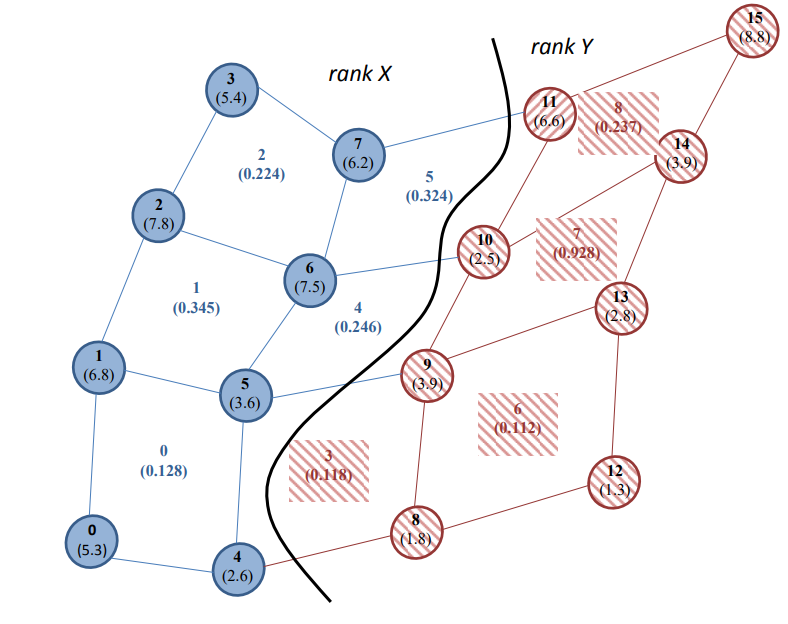
\includegraphics[width=\linewidth]{mesh_diagram.png}
    \caption{Mesh Partitioning Diagram \cite{mpi-dev}}
    \label{fig:mesh_partitioning}
\end{figure}
%Each rank is a different process, the halo edges would be the set $\{2, 5, 8, 9\}$, and the cells in the halos would be $\{0,3,4,5,7,8\}$. On top of splitting the sets into import/export halos, they can be further split into execute/non-execute lists based on whether the elements reference another in the same/different set. For example, in the figure above, edges $\{5,8,9\}$ would be part of X's exec import list because they reference cells $\{3,7,8\}$ in rank, whereas cells $\{3,7,8\}$ would be part of the non-exec import list. This is shown in the table below:
Each rank is dealt with by a different process, and so each has to track its own halo. On top of the split between import/export, each halo is split into execute/non-execute segments. A table showing the import/export lists for rank X is below:
\begin{figure*}
    % figure* environment puts the figure across two columns
    % but doesn't support h or h!
    \centering
    \begin{tabular}{|l|l||ll|ll|}
        \hline
        \multicolumn{1}{|c|}{Set Type} & \multicolumn{1}{c||}{Core} & \multicolumn{2}{c|}{Export Halo} & \multicolumn{2}{c|}{Import Halo} \\
                                      &                           & Execute       & Non-Execute      & Execute         & Non-Execute    \\ \hline
        Cells                          & \{0, 1, 2\}         & \{4, 5\}          & \{\}      & \{3\}            & \{\}    \\ \hline
        Nodes                          & \{0, 1, 2, 3, 4, 5, 6, 7\}         & \{\}         & \{4, 5, 6, 7\}             & \{\}     & \{8, 9, 10, 11\}           \\ \hline
    \end{tabular}
    \caption{Import/export halos for Rank X}
    \label{fig:Halo_set_example_table}
\end{figure*}
Note that Rank Y's export halo is the same as X's import halo shown above. This would not be the case if Rank X shared a boundary with another partition, but due to the simplicity of the example, X and Y's halos are mirrors of each other.

Core elements are ones that do not require any inter-process communication to compute. Therefore, a core element is any that only references other core elements. Above, it can be seen that only cells 0,1,2 are core to X, as 4 and 5 both reference elements in rank Y.

Export execute elements are ones that have at least one element that they reference that is not core to the process. Conversely, export non-execute elements are ones that are referenced by an element located on a foreign process (and that are not already in the execute list). The distinction here is that operations on an export exec element may update values in the other process, whereas non-exec elements are just required so the other process can carry out the computations in the first place.

Import execute elements are similar to export execute elements, but are for the current process. An element is an import execute element if it is referenced by another element in a foreign process, as the computation must be run on the foreign element to update the referenced local element. Similarly, import non-execute elements are just any foreign element that is referenced by local element (but not in the execute list), as the values will be needed to carry out the computation on the local element. 

In the MPI version, this exec/non-exec split is done so that non-blocking MPI primitives can be used, allowing for overlapping communication and computation. With PGAS, although the communication should be more efficient, it will still not be instant and so this exec/non-exec split will still be useful in this project. % I'm not sure this is correct, pretty sure non-exec/exec split is a validity thing right?

\subsubsection{Compute Loops} %TODO ben help with this as you know the MPI dev doc best. 

% In OP2, the performance of the application is critically dependent on the performance of the implementation of the primary compute loops. Thus each iteration is structured to maximise parallelism across the system, including between the compute and network units. 
The bulk of OP2's runtime comprises of compute loops that run user defined kernels to perform computation on sets and mappings with respect to user specified arguments. These loops can be either direct or indirect, relating to their direct or indirect reference to datasets (``If a [loop] consists of at least one [argument] that is indirectly accessed the whole loop is classified as an indirect loop'').

Under MPI, when a loop is called it is executed on each MPI process over the local elements of the set, as well as the \textit{import execute halo} if it is an indirect loop. Depending on certain factors, halo exchanges may be necessary before certain computation, and afterwards halos may need to be marked as ``dirty'' so they can be updated. Therefore a compute loop is essentially structured as follows, with parentheses denoting conditional steps:
\begin{enumerate}
    \item Begin halo exchange if necessary by exporting halo values
    \begin{itemize}
        \item This involves a non-blocking send operation, allowing the sender to return whilst the contents are still `in flight'. This enables parallelism of computation and network processing to increase system performance.
    \end{itemize}
    \item Perform computation on core elements
    \begin{itemize}
        \item This is the bulk of the computational operation.
    \end{itemize}
    \item Wait for import of halo values and perform computation on them
    \begin{itemize}
        \item This is the counterpart to the first export halo values in which this process now waits for the incoming import set values to arrive before continuing.
        \item Given the structure of the iteration, this information has hopefully already arrived given the network/compute parallelism such that the wait is not necessary. 
    \end{itemize}
    \item Mark halos as dirty if necessary
    \begin{itemize}
        \item This is done so that ``the next iteration of the loop can make the decision to update the halos as required''\cite{mpi-dev}.
    \end{itemize}
\end{enumerate}

%Something about how now as you can see the work is v fast n shit. 


\subsection{Configuration and Compilation}

% Supported hardware and libraries, what's optional and how it affects capabilities
The design of OP2 is centered around the idea of splitting the mesh computation implementation into two parts: Programs written by scientists solving high-level domain-specific problems which are agnostic to the hardware; and the implementation level of the OP2 library which is specific to the hardware used. OP2 can support  specific features of the hardware it's implemented for, for example Nvidia Kepler or Fermi graphic cards. These details and optimisations are, by design, invisible to the user as they do not need to consider them when using the library.

OP2 has a number of optional and non-optional dependencies. Notable ones include:
\begin{itemize}
    \item \textbf{HDF5} -- Used for handling of HDF files. Allows for scalable multi-threaded import of the mesh into memory and provides naïve partitioning. When absent, only \texttt{.dat} files can be used as a source of meshes and reading the mesh into memory is not parallelised.
    \item \textbf{PT-Scotch} and/or \textbf{ParMETIS} -- Used for optimised mesh partitioning. In case the libraries are absent, naïve partitioning is used.
    \item \textbf{CUDA} -- Used for running on CUDA-capable Nvidia GPUs. Also enables working with non-homogeneous nodes, for example a graphic card and two CPUs.
    \item \textbf{An MPI implementation} -- Enables running OP2 programs on distributed memory clusters. Our initial test run used OpenMPI. 
    \item \textbf{A Fortran compiler} -- To support the Fortran keybindings.
\end{itemize}

%Makefiles
The configuration of the library, including checks for existence of optional dependencies is done through an extensive Makefile infrastructure. The two main Makefiles, detecting all the dependencies and defining some compilation and build options accordingly are \texttt{common.mk} and \texttt{c\_app.mk}. In most cases, while developing own program with OP2, it is sufficient to include these two files (\texttt{c\_app}, as the name suggests, is intended for programs written in C, Fortran has a separate Makefile) into the program's Makefile and utilise variables provided. The global makefiles, such as the main ones described, are located in the \texttt{makefiles} folder. The makefiles specific to example applications are located in their respective directories. It is crucial to note that build options specific for building the OP2 library itself are defined in a makefile located in the \texttt{op2} folder together with the library implementation. 

\subsection{OP2 Preprocessor}\label{op2_implementation_notes}

% Division into folders, key briefly described.
% I incoprporated the  file and function locations into the discussion above

% IMportance of inlined functions and where translators
One of the key properties of the OP2 library distinct from its predecessor OPlus, is the preprocessor. It is most important when the code is prepared for execution on GPUs, as it defines when exactly the data is fetched between the system's memory and the graphic card's memory as well as accounting for platform-specific differences in the architecture of shared memory. It also processes indirect datasets to identify more optimal arrangement to store and access the data during runtime. The translator is a Python script and its files are located in the \texttt{translator} folder. 

% As an interesting sidenote, multiple functions including the main parallel loop implementation are defined as inline functions in header files. This is because inline functions do not create another layer on the execution stack, but rather are included directly into their parent function. This increases performance and assists compiler optimisations at the expense of a larger executable size. 

% %Fortran - plan to diregard it for now and trat with lower priority
% As it may have already become apparent from the sections above, the Fortran keybindings are treated as supplementary and the priority is to make the C bindings fully operational before attempting to supplement our work with Fortran support, should it require any modifications to the existing function bindings. This is due to the fact that the library itself is implemented in C/C++ and none of the team members is familiar with  Fortran. We recognise that a non-negligible part of the industry prefers Fortran for the kind of computations that are performed by OP2 and we are not ruling out ensuring compatibility eventually. 
